\documentclass{standalone}
\usepackage{pgfplots}
\pgfplotsset{compat=1.17}
\begin{document}
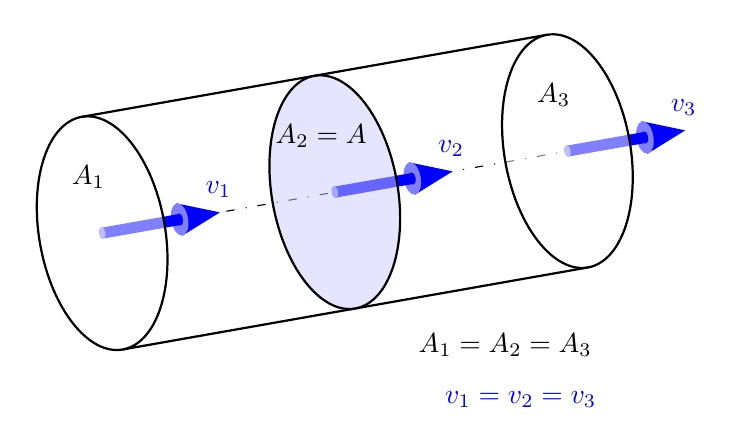
\begin{tikzpicture}[
bluedisc/.style={thick,fill=blue!20!white},
rest/.style={thick},
middleline/.style={loosely dash dot},
windarrow/.style={line width=4pt, blue}]

\begin{scope}[rotate=10]

\colorlet{bluedisc}{blue!20!white}
\colorlet{lightblue}{blue!50!white}

\draw[middleline] (0,0) -- (6,0);
\draw[rest] (0,1.5) -- (6,1.5);
\draw[rest] (0,-1.5) -- (6,-1.5);


\filldraw[blue] (1.5,0) -- (1,0.2) -- (1,-0.2) -- cycle;
    \filldraw[lightblue] (1,0) ellipse (.1 and .2);
    \draw[windarrow] (0,0) -- (1,0);
    \filldraw[lightblue] (0,0) ellipse (1pt and 2pt);
    \filldraw[blue] (1,0) ellipse (1pt and 2pt);
    \draw[windarrow] (0,0) (1.5,0) node[above] {$v_1$};
    
\filldraw[blue] (4.5,0) -- (4,0.2) -- (4,-0.2) -- cycle;
    \filldraw[lightblue] (4,0) ellipse (.1 and .2);
    \draw[windarrow] (3,0) -- (4,0);
    \filldraw[lightblue] (3,0) ellipse (1pt and 2pt);
    \filldraw[blue] (4,0) ellipse (1pt and 2pt);
    \draw[windarrow] (3,0) (4.5,0) node[above] {$v_2$};

\filldraw[blue] (7.5,0) -- (7,0.2) -- (7,-0.2) -- cycle;
    \filldraw[lightblue] (7,0) ellipse (.1 and .2);
    \draw[windarrow] (6,0) -- (7,0);
    \filldraw[lightblue] (6,0) ellipse (1pt and 2pt);
    \filldraw[blue] (7,0) ellipse (1pt and 2pt);
    \draw[windarrow] (6,0) (7.5,0) node[above] {$v_3$};

\draw[rest,fill=white,fill opacity=.5] (0,0) ellipse (.8 and 1.5);
\draw[rest,fill=bluedisc,fill opacity=.5] (3,0) ellipse (.8 and 1.5);
\draw[rest,fill=white,fill opacity=.5] (6,0) ellipse (.8 and 1.5);

\draw (0,1) node[anchor=north] {$A_1$};
\draw (3,1) node[anchor=north] {$A_2=A$};
\draw (6,1) node[anchor=north] {$A_3$};

\draw (6,-2.5) node[anchor=east] {$A_1 = A_2 = A_3$};
\draw[windarrow] (6,-3.2) node[anchor=east] {$v_1 = v_2 = v_3$};

\end{scope}
\end{tikzpicture}
\end{document}